\documentclass[11pt, oneside]{article}
\usepackage[letterpaper, margin=2cm]{geometry}
\usepackage{MATH517}

\begin{document}
\noindent \textbf{\Large{Caleb Logemann \\
MATH 517 Finite Difference Methods \\
Homework 1
}}

%\lstinputlisting[language=Matlab]{H01_23.m}
\begin{enumerate}
    \item % #1 Done
        Consider a nonuniform grid $x_1 < x_2 < x_3 < x_4$.
        Derive a finite difference approximation of $u''(x_2)$ that is as
        accurate as possible for smooth functions $u(x)$, based on the four
        values $U_1 = u(x_1)$, $U_2 = u(x_2)$, $U_3 = u(x_3)$, and
        $U_4 = u(x_4)$.
        Give an expression for the dominant term in the error.

        First let $h_1 = x_2 - x_1$, $h_2 = x_3 - x_2$ and $h_3 = x_4 - x_3$.
        In order to approximate $u''(x_2)$, we will use a linear combination of
        $U_1, \ldots, U_4$, that is we will find coefficients
        $\omega_1, \ldots, \omega_4$ such that
        $\omega_1 U_1 + \omega_2 U_2 + \omega_3 U_3 + \omega_4 U_4 = u''(x_2) + E$,
        where the error, $E$, is as small as possible.

        $U_1, U_3,$ and $U_4$ can be expressed as Taylor expansions about $U_2$
        as follows
        \begin{align*}
            U_1 &= u(x_1) = u(x_2) + u'(x_2)\p{-h_1} + \frac{1}{2} u''(x_2)
                \p{-h_1}^2 + \frac{1}{6} u'''(x_2) \p{-h_1}^3 +
                \frac{1}{24} u^{(4)}(c_1) \p{-h_1}^4 \\
            U_3 &= u(x_1) = u(x_2) + u'(x_2)\p{h_2} + \frac{1}{2} u''(x_2)
                \p{h_2}^2 + \frac{1}{6} u'''(x_2) \p{h_2}^3 +
                \frac{1}{24} u^{(4)}(c_2) \p{h_2}^4 \\
            U_4 &= u(x_1) = u(x_2) + u'(x_2)\p{h_2 + h_3} + \frac{1}{2} u''(x_2)
                \p{h_2 + h_3}^2 + \frac{1}{6} u'''(x_2) \p{h_2 + h_3}^3 +
                \frac{1}{24} u^{(4)}(c_3) \p{h_2 + h_3}^4
        \end{align*}
        where $c_1 \in \br{x_1, x_2}$, $c_2 \in \br{x_2, x_3}$, and
        $c_3 \in \br{x_2, x_4}$.

        Substituting these Taylor expansions into the linear combination and
        gathering the function and derivative values of $u$ at $x_2$ results in
        \begin{align*}
            \omega_1 U_1 + \omega_2 U_2 + \omega_3 U_3 + \omega_4 U_4 &=
                \p{\omega_1 + \omega_2 + \omega_3 + \omega_4} u(x_2) \\
                &+ \p{-h_1 \omega_1 + h_2 \omega_3 + \p{h_2 + h_3} \omega_4} u'(x_2) \\
                &+ \frac{1}{2}\p{h_1^2 \omega_1 + h_2^2 \omega_3 + \p{h_2 + h_3}^2 \omega_4} u''(x_2) \\
                &+ \frac{1}{6}\p{-h_1^3 \omega_1 + h_2^3 \omega_3 + \p{h_2 + h_3}^3 \omega_4} u'''(x_2) \\
                &+ \frac{1}{24}\p{h_1^4 \omega_1 u^{(4)}(c_1) + h_2^4 \omega_3 u^{(4)}(c_2)+ \p{h_2 + h_3}^4 \omega_4 u^{(4)}(c_3)}
        \end{align*}

        Since there are four coefficients to set in the linear combination we can
        specify up to 4 conditions on these coefficients to get the best possible
        approximation of $u''(x_2)$.
        These equations are as follows
        \begin{align*}
            \omega_1 + \omega_2 + \omega_3 + \omega_4 &= 0 \\
            -h_1 \omega_1 + h_2 \omega_3 + \p{h_2 + h_3} \omega_4 &= 0 \\
            h_1^2 \omega_1 + h_2^2 \omega_3 + \p{h_2 + h_3}^2 \omega_4 &= 2 \\
            -h_1^3 \omega_1 + h_2^3 \omega_3 + \p{h_2 + h_3}^3 \omega_4 &= 0
        \end{align*}
        If these equations are satisfied, then
        \begin{align*}
            \omega_1 U_1 + \omega_2 U_2 + \omega_3 U_3 + \omega_4 U_4 &= u''(x_2) + \frac{1}{24}\p{h_1^4 \omega_1 u^{(4)}(c_1) + h_2^4 \omega_3 u^{(4)}(c_2)+ \p{h_2 + h_3}^4 \omega_4 u^{(4)}(c_3)}
        \end{align*}
        where the approximation is $\omega_1 U_1 + \omega_2 U_2 + \omega_3 U_3 + \omega_4 U_4$
        and the error is \\
        $\frac{1}{24}\p{h_1^4 \omega_1 u^{(4)}(c_1) + h_2^4 \omega_3 u^{(4)}(c_2)+ \p{h_2 + h_3}^4 \omega_4 u^{(4)}(c_3)}$

        Using Mathematica, this system of equations can be solved, to find that
        the coefficients are
        \begin{align*}
            \omega_1 &= \frac{2\p{2 h_2 + h_3}}{h_1 \p{h_1 + h_2}\p{h_1 + h_2 + h_3}} \\
            \omega_2 &= \frac{2h_1 - 4 h_2 - 2 h_3}{h_1 h_2^2 + h_1 h_2 h_3} \\
            \omega_3 &= \frac{2\p{-h_1 + h_2 + h_3}}{h_2\p{h_1 + h_2} h_3} \\
            \omega_4 &= \frac{2\p{h_1 - h_2}}{h_3\p{h_2 + h_3}\p{h_1 + h_2 + h_3}}
        \end{align*}

        Since $u$ is a smooth function, the error can be simplified using the
        Intermediate Value Theorem, by noting that
        \begin{align*}
            \frac{h_1^4 \omega_1 u^{(4)}(c_1) + h_2^4 \omega_3 u^{(4)}(c_2)}{h_1^4 \omega_1 + h_2^4 \omega_3} &= u^{(4)}(\rho) \\
            h_1^4 \omega_1 u^{(4)}(c_1) + h_2^4 \omega_3 u^{(4)}(c_2) &= \p{h_1^4 \omega_1 + h_2^4 \omega_3} u^{(4)}(\rho)
        \end{align*}
        for some $\rho \in \br{x_1, x_3}$.
        Thus the error becomes
        \begin{align*}
            \frac{1}{24}\p{\p{h_1^4 \omega_1 + h_2^4 \omega_3}u^{(4)}(\rho)+ \p{h_2 + h_3}^4 \omega_4 u^{(4)}(c_3)}.
        \end{align*}
        The Intermediate Value Theorem can be used again to see that
        \begin{align*}
            \frac{\p{h_1^4 \omega_1 + h_2^4 \omega_3}u^{(4)}(\rho)+ \p{h_2 + h_3}^4 \omega_4 u^{(4)}(c_3)}{h_1^4 \omega_1 + h_2^4 \omega_3 + \p{h_2 + h_3}^4 \omega_4} &= u^{(4)}(\mu) \\
            \p{h_1^4 \omega_1 + h_2^4 \omega_3}u^{(4)}(\rho)+ \p{h_2 + h_3}^4 \omega_4 u^{(4)}(c_3) &= \p{h_1^4 \omega_1 + h_2^4 \omega_3 + \p{h_2 + h_3}^4 \omega_4} u^{(4)}(\mu)
        \end{align*}
        for $\mu \in \br{x_1, x_4}$.

        The error can thus be written as
        \begin{align*}
            E &= \frac{1}{24}\p{h_1^4 \omega_1 + h_2^4 \omega_3 + \p{h_2 + h_3}^4 \omega_4} u^{(4)}(\mu).
        \end{align*}
        Substituting in for $\omega_1$, $\omega_3$, and $\omega_4$ and
        simplifying results in
        \begin{align*}
            E &= -\frac{1}{12} \p{h_2\p{h_2 + h_3} - h_1 \p{2 h_2 + h_3}} u^{(4)}(\mu).
        \end{align*}

    \item % #2 Done
    \item % #3 Done
        The script for problems 2 and 3 is shown below with output shown after that.
        \lstinputlisting[language=Matlab]{H01_23.m}
        \begin{center}
            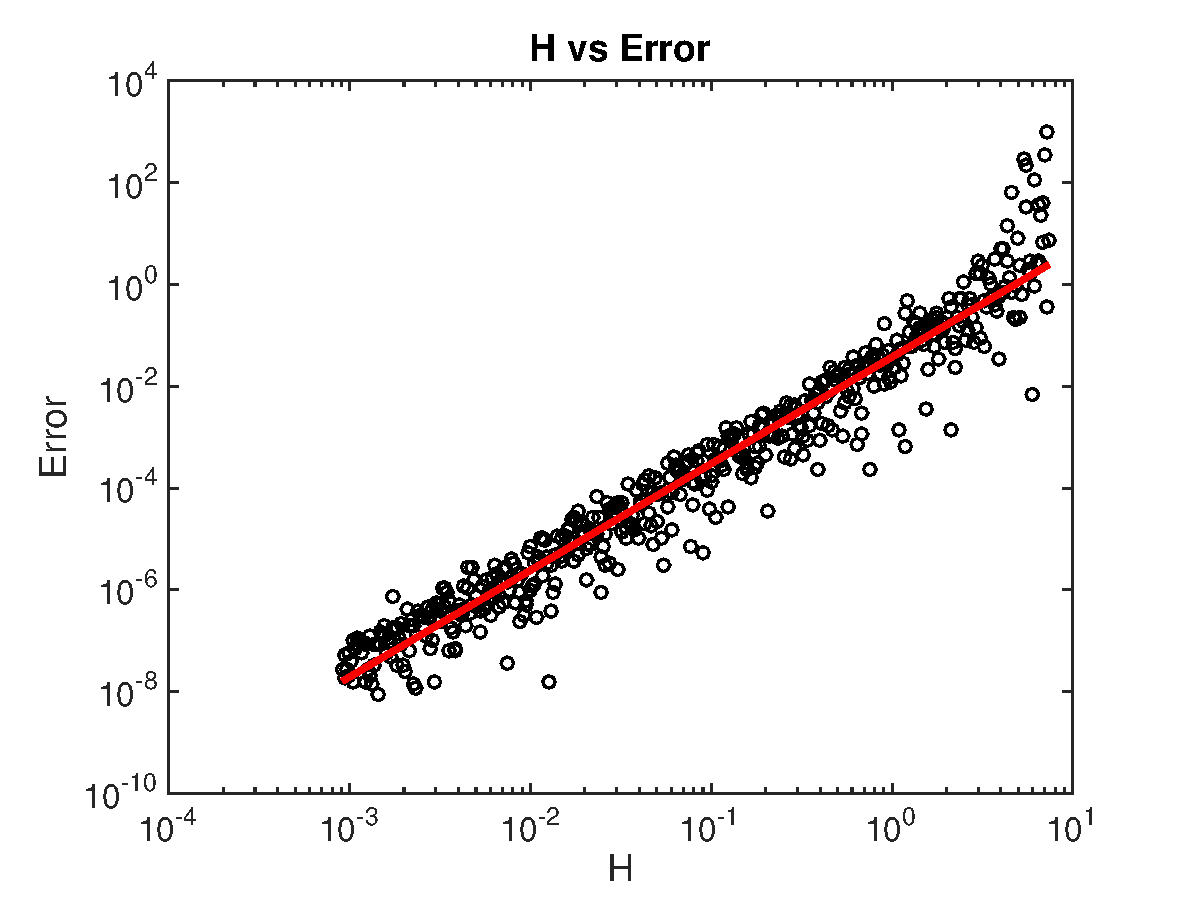
\includegraphics[scale=.5]{Figures/01_1.eps}
        \end{center}
        \begin{verbatim}
            >> H01_23

            p =

                2.0956


            K =

                -3.2838
        \end{verbatim}

    \item % #4 Done
        Consider the following 2-pt BVP:
        \begin{align*}
            u'' + u = f(x), \quad \text{on} \quad 0 \le x \le 10 \\
            u'(0) - u(0) = 0, \quad u'(10) + u(10) = 0
        \end{align*}
        Construct a second order accurate finite-difference method for this BVP.
        Write your method as a linear system in the form $A \v{u} = \v{f}$.

        First the interval $\br{0, 10}$ needs to be discretized.
        Let $x_0 = 0$, $x_{N + 1} = 10$, and let $x_{i} = ih$ for $1 \le i \le N$,
        where $h = \frac{10}{N+1}$.
        Thus the interval $\br{0, 10}$ is described as a grid of $N+2$ equally
        spaced points with grid spacing $h$.
        Thus the solution to this BVP will be approximated on these grid points.
        Let $U_i$ be the approximate value of $u(x_i)$.
        Thus an approximate solution to this BVP will be the values of $U_i$ for
        $0 \le i \le N+1$.

        Based on the boundary conditions be can find expressions for $U_0$ and
        $U_{N+1}$.
        The first boundary condition states that
        \begin{align*}
            u'(0) - u(0) = 0
        \end{align*}
        We can approximate $u'(0)$ with a second order finite difference.
        \begin{align*}
            u'(0) \approx \frac{-\frac{1}{2}U_2 + 2U_1 - \frac{3}{2}U_0}{h}
        \end{align*}
        Thus the boundary condition can be rewritten in terms of the
        discretization as follows
        \begin{align*}
            -\frac{1}{2}U_2 + 2U_1 - \frac{3}{2}U_0 - hU_0 &= 0 \\
            U_0 &= \p{4U_1 - U_2} \frac{1}{3 + 2h}
        \end{align*}
        The second boundary condition can be similarly manipulated.
        \begin{align*}
            u'(10) + u(10) &= 0 \\
            u'(10) &\approx  \frac{\frac{3}{2}U_{N+1} - 2U_N + \frac{1}{2}U_{N-1}}{h}\\
            \frac{3}{2}U_{N+1} - 2U_N + \frac{1}{2}U_{N-1} + hU_{N+1} &= 0 \\
            U_{N+1} &= \p{4U_N - U_{N-1}} \frac{1}{3 + 2h}
        \end{align*}

        Now that expressions for $U_0$ and $U_{N+1}$ have been found, we can
        find $N$ equations for the remaining $N$ unkowns, $U_{i}$ for
        $1 \le i \le N$.
        In order that the finite-difference method is second order accurate, I
        will use the second order central difference to approximate the second
        derivative.
        This finite difference is
        \begin{align*}
            u''(x_i) \approx \frac{1}{h^2}\p{U_{i-1} - 2U_{i} + U_{i+1}}
        \end{align*}
        for $1 \le i \le N$.

        This finite difference can then be used in the differential equation to
        create $N$ equations as follows
        \begin{align*}
            \frac{1}{h^2}\p{U_{i-1} - 2U_{i} + U_{i+1}} + U_i &= f(x_i) \\
            \frac{1}{h^2}\p{U_{i-1} + (-2 + h^2)U_{i} + U_{i+1}} &= f(x_i)
        \end{align*}
        for $2 \le i \le N - 1$.
        For $i = 1$ and $i = N$, we need to substitute the expression for $U_0$
        and $U_{N+1}$ respectively.
        This results in
        \begin{align*}
            f(x_1) &= \frac{1}{h^2}\p{\p{4U_1 - U_2} \frac{1}{3 + 2h} - 2U_{1} + U_{2}} + U_1 \\
            f(x_1) &= \frac{1}{h^2}\p{\p{\frac{4}{3 + 2h} - 2 + h^2}U_1 + \p{1-\frac{1}{3 + 2h}}U_2} \\
            f(x_{N}) &= \frac{1}{h^2}\p{U_{N-1} - 2U_{N} + \p{4U_N - U_{N-1}} \frac{1}{3 + 2h}} + U_N \\
            f(x_{N}) &= \frac{1}{h^2}\p{\p{1 - \frac{1}{3 + 2h}}U_{N-1} + \p{\frac{4}{3 + 2h} - 2 + h^2}U_{N}}
        \end{align*}

        These $N$ equations can be expressed as the matrix equation
        \begin{align*}
            A\v{u} &= \v{f}
            \intertext{where}
            \v{u} &= \br{U_1, U_2, \cdots, U_N}^T \\
            \v{f} &= \br{f(x_1), f(x_2), \cdots, f(x_N)}^T \\
            A &= \frac{1}{h^2}
            \begin{bmatrix}
                \frac{4}{3 + 2h} -2 + h^2 & 1 - \frac{1}{3 + 2h} & & &  \\
                1 & -2 + h^2 & 1 & & \\
                  & \ddots & \ddots & \ddots & \\
                  &        & 1 & -2 + h^2 & 1 \\
                  &        &   & 1 - \frac{1}{3 + 2h} & \frac{4}{3 + 2h} -2 + h^2 \\
            \end{bmatrix}
        \end{align*}
        $A$ is a tridiagonal matrix, so all other entries are zero.
        Therefore to approximate the solution solve the system $A\v{u} = \v{f}$ and
        then plug in values for the expressions of $U_0$ and $U_{N+1}$.

    \item % #5 Done
        Construct the exact solution to the BVP with $f(x) = -e^x$.

        This is a nonhomogenous ODE, so the solution to this BVP is found
        by summing the solutions to the homogenous and nonhomogenous equations.
        First I will begin by solving the homogenous version of the BVP, which
        is
        \begin{align*}
            u'' + u = 0
        \end{align*}
        It is known that the general solution to this homogenous ODE is of the
        form
        \begin{align*}
            u(x) &= a\sin{x} + b\cos{x} \\
            u''(x) &= -a\sin{x} - b\cos{x}
        \end{align*}
        which clearly satisfies the homogenous ODE.

        A solution to the nonhomogenous ODE can be found as well.
        In this case the ODE is
        \begin{align*}
            u'' + u = -e^x
        \end{align*}
        I will guess that the solution is of the form
        \begin{align*}
            u(x) &= c_1 e^x + c_2 e^{-x} \\
            u''(x) &= c_1 e^x + c_2 e^{-x}.
            \intertext{Substituting this into the ODE results in}
            2c_1 e^x + 2c_2 e^{-x} &= -e^x.
            \intertext{Therefore}
            c_1 &= -\frac{1}{2} \\
            c_2 &= 0
            \intertext{Thus the nonhomogenous solution is}
            u(x) &= -\frac{1}{2}e^x
        \end{align*}
        Therefore the overall solution to this BVP is
        \begin{align*}
            u(x) &= -\frac{1}{2}e^x + a\sin{x} + b\cos{x}
        \end{align*}

        Finally we must find $a$ and $b$ such that $u(x)$ satisfies the
        boundary conditions.
        \begin{align*}
            u'(x) &= -\frac{1}{2}e^x + a\cos{x} - b\sin{x} \\
            u(0) &= -\frac{1}{2} + b \\
            u'(0) &= -\frac{1}{2} + a \\
            0 &= u'(0) - u(0) \\
            &= -\frac{1}{2} + a + \frac{1}{2} - b \\
            a &= b \\
            u(10) &= -\frac{1}{2}e^{10} + a\sin{10} + b\cos{10} \\
            u'(10) &= -\frac{1}{2}e^{10} + a\cos{10} - b\sin{10} \\
            0 &= u'(10) + u(10) \\
              &= -e^{10} + \p{\cos{10} + \sin{10}}a + \p{\cos{10} - \sin{10}}b
            \intertext{Substituting in $a$ for $b$.}
            0 &= -e^{10} + 2\cos{10}a \\
            a &= \frac{e^{10}}{2\cos{10}} \\
            b &= \frac{e^{10}}{2\cos{10}} \\
        \end{align*}
        Therefore the exact solution to the BVP is
        \begin{align*}
            u(x) &= -\frac{1}{2}e^x + \frac{e^{10}}{2\cos{10}}\p{\sin{x} + \cos{x}}
        \end{align*}

    \item % #6 Done
        Verify that your method is second order accurate by solving the BVP with
        $f(x) = -e^x$ for four different grid spacings $h$.

        The script for solving this BVP is shown below.
        \lstinputlisting[language=Matlab]{H01_6.m}
        This outputs the following, which shows that as $h$ decreases by
        a factor of $2$ the error decreases by a factor of $4$ which
        shows that the method is of order $2$.
        \begin{verbatim}
            >> H01_6

            ans = 

                hRatios    errorRatios    order 
                _______    ___________    ______

                1.9091     3.6953         2.0214
                1.9524     3.5994         1.9143
                1.9756     3.7616         1.9458
                1.9877     3.8869         1.9763
                1.9938     3.9406         1.9873
                1.9969     3.9697         1.9935
                1.9984     3.9849         1.9968
                1.9992     3.9924         1.9984
                1.9996     3.9963         1.9992
        \end{verbatim}

    \item % #7 Done
        Consider the following 2-point BVP:
        \begin{align*}
            -u'' + u = f(x), \quad \text{on} \quad 0 \le x \le 1 \\
            u(0) = u(1) \quad u'(0) = u'(1)
        \end{align*}
        Construct a fourth-order accurate finite-difference method for this BVP
        based on the fourth-order central finite difference.
        Write your method as a linear system of the form $A\v{u} = \v{f}$.

        First the interval $\br{0, 1}$ needs to be discretized.
        Let $x_0 = 0$, $x_{N + 1} = 1$, and let $x_{i} = ih$ for $1 \le i \le N$,
        where $h = \frac{1}{N+1}$.
        Thus the interval $\br{0, 1}$ is described as a grid of $N+2$ equally
        spaced points with grid spacing $h$.
        Thus the solution to this BVP will be approximated on these grid points.
        Let $U_i$ be the approximate value of $u(x_i)$.
        Thus an approximate solution to this BVP will be the values of $U_i$ for
        $0 \le i \le N+1$.

        The boundary conditions are periodic, this implies that we can use the
        following equalities
        \begin{align*}
            U_0 &= U_{N+1} \\
            U_{-1} &= U_{N} \\
            U_{-2} &= U_{N-1} \\
            U_{N+2} &= U_1 \\
        \end{align*}
        The periodic boundary conditions reduces the number of unknowns from
        $N+2$ to $N+1$, and it allows for the finite difference to be
        used at all points $i = 0, 1, \ldots, N$.

        In order that this method is fourth-order accurate, I will use the
        fourth-order central difference to approximate the second derivative,
        which is
        \begin{align*}
            u''(x_i) &\approx \frac{-U_{i-2} + 16U_{i-1} - 30U_i + 16U_{i+1} - U_{i+2}}{12h^2}
        \end{align*}

        Therefore the finite difference equation for this differential equations
        is
        \begin{align*}
            \frac{U_{i-2} - 16U_{i-1} + \p{30 + 12h^2}U_i - 16U_{i+1} + U_{i+2}}{12h^2} = f(x_i)
        \end{align*}
        for $i = 0, 1, \ldots, N$.

        This is equivalent to the following matrix equation
        \begin{align*}
            A\v{u} &= \v{f}
            \intertext{where}
            \v{u} &= \br{U_0, U_1, \cdots, U_N}^T \\
            \v{f} &= \br{f(x_0), f(x_1), \cdots, f(x_N)}^T \\
            A &= \frac{1}{12h^2}
            \begin{bmatrix}
                30+12h^2 & -16    & 1      &        & \cdots & 1      & -16 \\
                -16    & 30+12h^2 & -16    & 1      &        & \cdots & 1   \\
                1      & -16    & 30+12h^2 & -16    & 1      &        &     \\
                \vdots & \ddots & \ddots & \ddots & \ddots & \ddots & \vdots \\
                       &        & 1      & -16    & 30+12h^2 & -16    & 1   \\
                1      & \cdots &        & 1      & -16    & 30+12h^2 & -16 \\
                -16    & 1      & \cdots &        & 1      & -16     & 30+12h^2 \\
            \end{bmatrix}
        \end{align*}

    \item % #8 Done
        Construct an exact solution to the BVP for $f(x) = \sin{4\pi x}$.

        As we have seen the exact solution to this BVP will be the sum of the
        homogenous solution, $u_h$, and nonhomogenous solution, $u_n$, to this BVP.
        The homogenous version of this BVP is
        \begin{align*}
            -u_h'' + u_h = 0.
        \end{align*}
        The solution to this ODE is of the form $u_h(x) = a\sin{x} + b\cos{x}$.

        The nonhomogenous solution can be found as follows.
        First I will guess that the solution is of the form
        $u_n(x) = c_1 \sin{4\pi x} + c_2\cos{4 \pi x}$.

        The constants in this function can be found by
        plugging this function into the differential equation.
        \begin{align*}
            u_n''(x) &= -16 \pi^2 c_1 \sin{4\pi x} - 16 \pi^2 c_2 \cos{4 \pi x} \\
            \sin{4 \pi x} &= -u_n''(x) + u_n(x) \\
                          &= \p{16 \pi^2 + 1} c_1 \sin{4\pi x} + \p{16 \pi^2 + 1} c_2 \cos{4 \pi x}
            \intertext{This results in the following two equations}
            1 &= \p{16 \pi^2 + 1} c_1 \\
            c_1 &= \frac{1}{16 \pi^2 + 1} \\
            0 &= \p{16 \pi^2 + 1} c_2 \\
            c_2 &= 0
        \end{align*}
        Thus the nonhomogenous solution to this BVP is
        $u_n(x) = \frac{1}{16\pi^2 + 1} \sin{4\pi x}$.

        Therefore the full solution is of the form
        $u(x)=a\sin{x} + b\cos{x} + \frac{1}{16\pi^2 + 1} \sin{4\pi x}$.
        Now we must select $a$ and $b$ to satisfy the periodic boundary conditions.

        \begin{align*}
            u(x) &= a\sin{x} + b\cos{x} + \frac{1}{16\pi^2 + 1} \sin{4\pi x} \\
            u(0) &= b \\
            u(1) &= a\sin{1} + b\cos{1} \\
            u(0) &= u(1) \\
            b    &= a\sin{1} + b\cos{1} \\
            a    &= \p{\frac{1 - \cos{1}}{\sin{1}}}b \\
            u'(x) &= a\cos{x} - b\sin{x} + \frac{4\pi}{16\pi^2 + 1} \cos{4\pi x} \\
            u'(0) &= a + \frac{4\pi}{16\pi^2 + 1} \\
            u'(1) &= a\cos{1} - b\sin{1} + \frac{4\pi}{16\pi^2 + 1} \\
            u'(0) &= u'(1) \\
            a + \frac{4\pi}{16\pi^2 + 1} &= a\cos{1} - b\sin{1} + \frac{4\pi}{16\pi^2 + 1} \\
            a &= a\cos{1} - b\sin{1} \\
            0 &= \p{\cos{1} - 1}a - b\sin{1}
            \intertext{Substituting for $a$}
            0 &= \p{\cos{1} - 1}\p{\frac{1 - \cos{1}}{\sin{1}}}b - \sin{1} b \\
            0 &= \p{\frac{-\cos{1}^2 + 2\cos{1} - 1 - \sin{1}^2}{\sin{1}}} b \\
            0 &= \p{\frac{2\cos{1} - 2}{\sin{1}}} b
            \intertext{Since $\frac{2\cos{1} - 2}{\sin{1}} \neq 0$, then}
            b &= 0
            \intertext{Therefore}
            a &= 0
        \end{align*}
        Thus the exact solution to the BVP is $u(x) = \frac{1}{16\pi^2 + 1} \sin{4\pi x}$.

    \item % #9 Done
        Verify that your method is fourth-order accurate by solving the BVP with
        $f(x) = \sin{4\pi x}$ at four different grid spacings h.

        \lstinputlisting[language=Matlab]{H01_9.m}
        \begin{verbatim}
            >> H01_9

            ans = 

                hRatios    errorRatios    order 
                _______    ___________    ______

                1.9091     12.309         3.8822
                1.9524      14.18         3.9636
                1.9756     15.132         3.9902
                1.9877     15.581         3.9975
                1.9938     15.794         3.9993
                1.9969     15.898         3.9998
                1.9984       14.9         3.9017
        \end{verbatim}

    \item % #10
        Prove that your method is consistent with truncation error
        $\norm{\v{\tau}} = O(h^4)$ and $L_2$-stable, thereby proving that
        your method converges at $O(h^4)$ in the $L_2$-norm.

        First I will prove that my method is consistent with fourth order
        accuracy.
        A method is considered consistent and fourth order accurate if the
        norm of the truncation error approaches zero at the same rate as $h^4$.
        The truncation error is defined as the difference between the 

        In this case the truncation error is
        \begin{align*}
            \tau_i &= \frac{1}{12h^2}\p{u(x_{i-2}) - 16u(x_{i-1}) + \p{30 + 12h^2}u(x_i) - 16u(x_{i+1}) + u(x_{i+2})} - f(x_i)
        \end{align*}
        \begin{align*}
            \intertext{This can be simplified using the following Taylor series}
            u(x_{i-2}) &= u(x_i) - 2hu'(x_i) + 2h^2u''(x_i) - \frac{4}{3}h^3u'''(x_i) + \frac{2}{3}h^4u^{(4)}(x_i) - \frac{4}{15}h^5u^{(5)}(x_i) + \frac{4}{45}h^6u^{(6)}(c_{-2}) \\
            -16u(x_{i-1}) &= -16 u(x_i) + 16hu'(x_i) - 8h^2u''(x_i) + \frac{8}{3}h^3u'''(x_i) - \frac{2}{3}h^4u^{(4)}(x_i) + \frac{2}{15}h^5u^{(5)}(x_i) - \frac{1}{45}h^6u^{(6)}(c_{-1}) \\
            -16u(x_{i+1}) &= -16 u(x_i) - 16hu'(x_i) - 8h^2u''(x_i) - \frac{8}{3}h^3u'''(x_i) - \frac{2}{3}h^4u^{(4)}(x_i) - \frac{2}{15}h^5u^{(5)}(x_i) - \frac{1}{45}h^6u^{(6)}(c_{1}) \\
            u(x_{i+2}) &= u(x_i) + 2hu'(x_i) + 2h^2u''(x_i) + \frac{4}{3}h^3u'''(x_i) + \frac{2}{3}h^4u^{(4)}(x_i) + \frac{4}{15}h^5u^{(5)}(x_i) + \frac{4}{45}h^6u^{(6)}(c_{2}) \\
        \end{align*}
        Adding these four Taylor series results in
        \begin{align*}
            u(x_{i-2}) - 16u(x_{i-1}) - 16u(x_{i+1}) + u(x_{i+2}) &= -30u(x_i) - 12 h^2 u''(x_i)  \\
            &+ \frac{1}{45}h^6\p{4u^{(6)}(c_{-2}) - u^{(6)}(c_{-1}) - u^{(6)}(c_{1}) + 4u^{(6)}(c_{2})}
            \intertext{The Intermediate Value Theorem can be used several times to simplify the final term}
            u(x_{i-2}) - 16u(x_{i-1}) - 16u(x_{i+1}) + u(x_{i+2}) &= -30u(x_i) - 12 h^2 u''(x_i) + \frac{6}{45}h^6u^{(6)}(\mu)
        \end{align*}
        Plugging this expression back into the truncation error formula results in
        \begin{align*}
            \tau_i &= \frac{1}{12h^2}\p{\p{30 + 12h^2}u(x_i) -30u(x_i) - 12 h^2 u''(x_i) + \frac{6}{45}u^{(6)}(\mu)} - f(x_i) \\
                   &= u(x_i) - u''(x_i) + \frac{1}{90}h^4u^{(6)}(\mu) - f(x_i)
            \intertext{Since $u$ is a solution to the differential equation, $f(x_i) = -u''(x_i) + u(x_i)$}
            \tau_i &= \frac{1}{90}h^4u^{(6)}(\mu)
            \intertext{Therefore}
            \tau_i &= O(h^4)
        \end{align*}
        This shows that our method is consistent and is fourth order accurate.

        In order to show that our method is $L_2$ stable, we must show that
        $\norm[2]{A^{-1}} \le C$.

        Since $A$ is symmetric we know that
        $\norm[2]{A^{-1}} = \rho(A^{-1}) = \frac{1}{\min{\lambda_i}}$, where
        $\lambda_i$ are the eigenvalues of $A$.
        To find the eigenvalues of $A$, we must first find the eigenfunctions

        of the original BVP, that is we must find functions $v$ that satisfy
        \begin{align*}
            -v'' + v = \lambda v, \quad \text{on} \quad 0 \le x \le 1 \\
            v(0) = 0 \quad v(1) = 0
        \end{align*}

        This is equivalent to the ODE
        \begin{align*}
            -v'' = (\lambda - 1)v
        \end{align*}
        The general solution to this ODE is
        \[
            v(x) = a\sin{\sqrt{\lambda - 1}x} + b\cos{\sqrt{\lambda - 1}x}
        \]
        Based on the boundary condition $v(0) = 0$
        \begin{align*}
            0 &= a\sin{0} + b\cos{0} \\
            b &= 0
            \intertext{and by the boundary condition $v(1) = 0$}
            0 &= a\sin{\sqrt{\lambda - 1}}
            \intertext{To find nontrivial solutions implies that}
            \sqrt{\lambda-1} &= n\pi \\
            \lambda &= n^2 \pi^2 + 1
        \end{align*}

        Therefore the eigenvalues of this continuous problem are $n^2 \pi^2 + 1$
        for $n = 1, 2, \ldots$, and the eigenfunctions are $v^p = \sin{p\pi x}$.

        Therefore for the continuous problem I will guess that the eigenvectors
        have the same form as the eigenvalues.
        Thus I will quess that the eigenvectors, $\v{v}^p$ of $A$ has entries
        $v^p_j = \sin{p\pi x_j} = \sin{p\pi jh}$, that is the eigenvectors
        are the eigenfunctions sampled on the mesh.
        To verify this we must compute the entries of $A\v{v}^p$.
        The jth entry of $A\v{v}^p$ can be found as follows
        \begin{align*}
            \p{A\v{v}^p}_j &= \frac{1}{12h^2}\p{v^p_{j-2} - 16v^p_{j-1} + \p{30 + 12h^2}v^p_j - 16v^p_{j+1} + v^p_{j+2}} \\
                           &= \frac{1}{12h^2}(\sin{p\pi(j-2)h} - 16\sin{p\pi(j-1)h} \\
                           &+ \p{30 + 12h^2}\sin{p\pi jh} - 16\sin{p\pi(j+1)h} + \sin{p\pi(j+2)h})
            \intertext{The following trigonometric identies can be used to simplify this expression}
            \sin{p\pi(j-2)h} &= \sin{p\pi jh}\cos{2p\pi h} - \cos{p\pi jh}\sin{2p\pi h} \\
            -16\sin{p\pi(j-1)h} &= -16\p{\sin{p\pi jh}\cos{p\pi h} - \cos{p\pi jh}\sin{p\pi h}} \\
            -16\sin{p\pi(j+1)h} &= -16\p{\sin{p\pi jh}\cos{p\pi h} + \cos{p\pi jh}\sin{p\pi h}} \\
            \sin{p\pi(j+2)h} &= \sin{p\pi jh}\cos{2p\pi h} + \cos{p\pi jh}\sin{2p\pi h}
            \intertext{Substituting these identities in and simplifying results in}
            \p{A\v{v}^p}_j &= \frac{1}{12h^2}\p{\p{30 + 12h^2}\sin{p\pi jh} + 2\sin{p\pi jh}\cos{2p\pi h} -32\sin{p\pi jh}\cos{p\pi h}} \\
                           &= \frac{1}{12h^2}\p{30 + 12h^2 + 2\cos{2p\pi h} - 32\cos{p\pi h}}\sin{p\pi jh} \\
                           &= \frac{1}{12h^2}\p{30 + 12h^2 + 2\cos{2p\pi h} - 32\cos{p\pi h}}v^p_j \\
        \end{align*}
        So this vector is indeed an eigenvector with eigenvalue
        \begin{align*}
            \lambda^p &= \frac{1}{12h^2}\p{30 + 12h^2 + 2\cos{2p\pi h} - 32\cos{p\pi h}}
            \intertext{Doing a Taylor series expansion on this eigenvalue results in}
            \lambda^p &\approx (1 + p^2 \pi^2) - \frac{1}{90}p^6 \pi^6 h^4 + O(h^6)
            \min{\lambda^p} &= \lambda^1 \approx (1 + \pi^2) - \frac{1}{90} \pi^6 h^4 + O(h^6)
        \end{align*}

        Coming back to our initial problem, we now know that
        \begin{align*}
            \norm[2]{A^{-1}} &= \rho(A^{-1}) \\
            &= \frac{1}{\lambda^1} \\
            &\le \frac{1}{1 + pi^2}
        \end{align*}
        Therefore the $\norm[2]{A^{-1}}$ is bounded and out method is
        $L_2$-stable.

\end{enumerate}
\end{document}
